\documentclass[a4paper,10pt]{report}
\usepackage[utf8x]{inputenc}
\usepackage[T1]{fontenc}
\usepackage[french]{babel} 
\usepackage{lmodern} % Pour changer le pack de police
\usepackage{makeidx}
\usepackage{graphicx}
\graphicspath{{figures/}}

\title{Projet 3A\\Analyse d'imagerie polarimétrique}
\author{\textsc{Guinaudeau} Alexandre\\
	\and 
	\textsc{Hulot} Pierre
	\and 
	\textsc{Dejoie} Etienne	
	}
\date{\today}
\makeindex
\begin{document}

\maketitle

\begin{abstract}
Le résumé (abstract en anglais) de mon article.
\end{abstract}

\chapter{contexte}
\section{ADM Polar, contexte du projet}
\section{Presentation des données}
 A mettre ici : présentation du set données. Nombre de pièces différentes. taille des images. Explication de ce qu'est la matrice de Muller


\chapter{Le traitement des données}

\section{Prétraitement des données}
Les différents types de prétraitements que l'on peut faire avant de traiter les données

\section{Les différentes approches de traitement des données}

\subsection{Réduction de dimension}
\subsubsection{PCA}
\paragraph{rappel de laméthode }
L'Analyse en Composantes Principales (ou PCA) consiste à essayer de représenter les données dans un espace de plus petites dimensions. Les vecteurs directeurs du nouvel espace maximise la variance entre les données. Nous présentons ici les résultats pour la dimension 2.
\paragraph{prétraitement utilisé}
Nous effectuaons cette PCA sur les centres des clusters préalablement présentés (cf 1.1.1). Les centres des clusters représentent de manière fidèle l'ensemble des points qu'il rassemble. Chaque cluster est représenté par un vecteur d'éléments de la matrice de Muller. Tous les éléments de Muller sont gardés à l'exeption de la première ligne et première colonne qui ne sont pas a priori pertinentes (d'après les informations des physiciens)
\begin{figure}
  \caption{centre des clusters avant transformation}
  \centering
  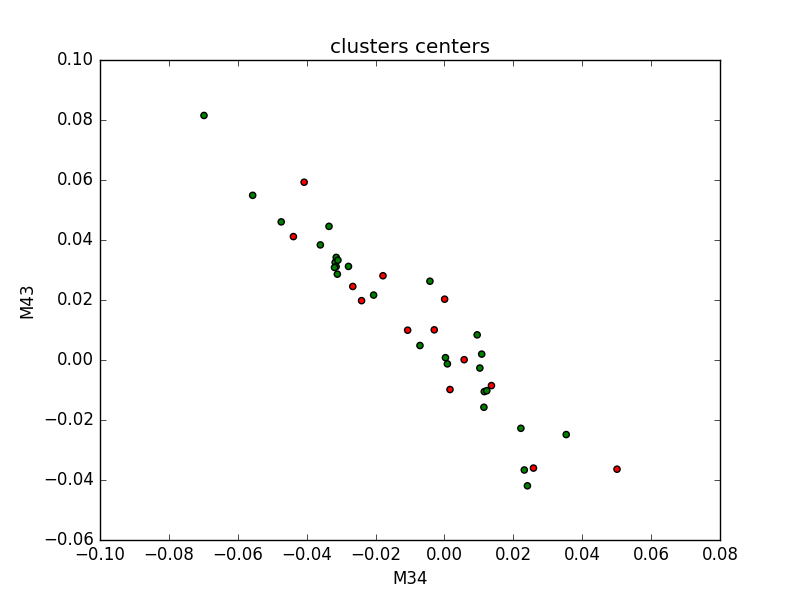
\includegraphics[width=10cm]{PCA_0.png}
\end{figure}
\begin{figure}
  \caption{centre des clusters après transformation}
  \centering
  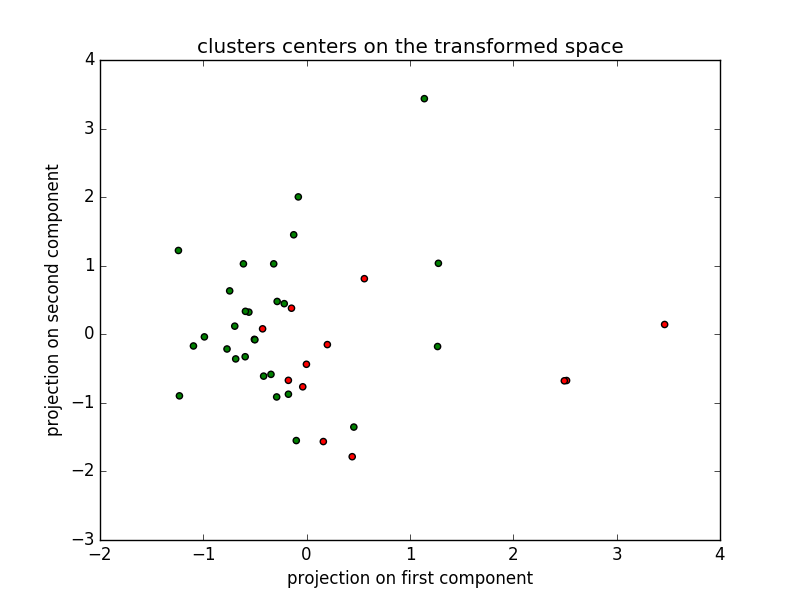
\includegraphics[width=10cm]{PCA_1.png}
\end{figure}
\begin{figure}
  \caption{Part de variance expliquée}
  \centering
  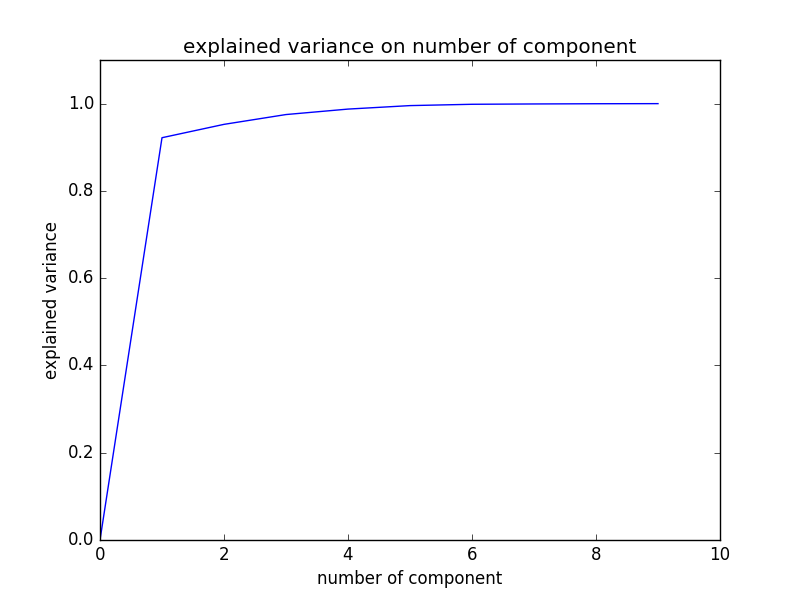
\includegraphics[width=10cm]{PCA_3.png}
\end{figure}
\begin{figure}
  \caption{analyse de la comosante principale}
  \centering
  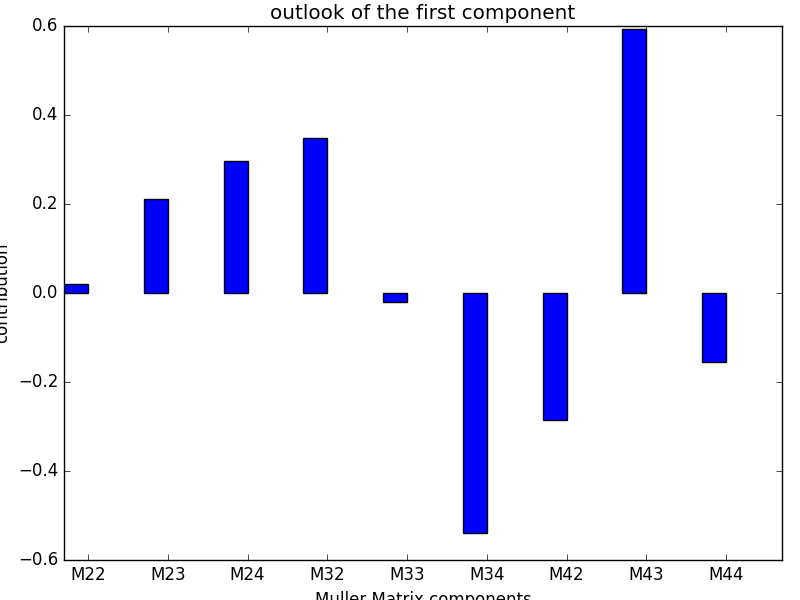
\includegraphics[width=10cm]{PCA_2.png}
\end{figure}

\paragraph{résultats}
La réduction de dimension par PCA semble efficace. La composante principale explique 90\% de la variance (fig 2.3). 
De l'analyse de la première comosante (fig 2.4) ressort deux effets principaux :
- La petite contribution des éléments diagonaux de la matrice de Muller
- Le rôle prépondérant de M34 et M43

On remarque une certaine anticorrlation des éléments de la matrice de muller. Le poids de M43 est proche de l'opposé de celui de M34. Le poids de M42 est également proche de l'opposé de celui de M24. Cette observation n'est par contre pas vérifiée pour M23 et M32 qui semblent corrélés.
\paragraph{conclusion}
La PCA effectuée sur les centres des clusters valident certaines supposition comme le rôle faible des éléments diagonaux ou le rôle improtant des éléments M34 et M43.

Par contre, la projection de la PCA en 2 dimensions ne nous permet pas de séparer les données de manière suffisantes pour être capable de distinguer des zones clairement différentes entre les clusters sains et les clusters malades. (fig 2.2)
\subsection{Méthode de classification}

\subsubsection{Arbre décisionnel et Random Forest}
\paragraph{rappel de laméthode }
\paragraph{prétraitement utilisé}
\paragraph{résultats (notamment graphique)}
\paragraph{explication}
\paragraph{piste d'amélioration}

\subsubsection{K plus proche voisin}
\paragraph{rappel de laméthode }
\paragraph{prétraitement utilisé}
\paragraph{résultats (notamment graphique)}
\paragraph{explication}
\paragraph{piste d'amélioration}

\tableofcontents


Bla\index{bla} bla bla

\listoffigures
\listoftables
\printindex
\end{document}
